\documentclass{article}

\usepackage[english]{babel}
\usepackage[letterpaper,top=2cm,bottom=2cm,left=3cm,right=3cm,marginparwidth=1.75cm]{geometry}
\usepackage{amsmath}
\usepackage{graphicx}
\usepackage{float}
\usepackage{booktabs}
\usepackage{textcomp}
\usepackage[colorlinks=true, allcolors=blue]{hyperref}

\title{Blink-DB: Design Document}
\author{
      Gana Jayant Sigadam \\
      Roll No: 24CS60R12 \\
}

\begin{document}
\maketitle

\section{Introduction}
This is the design document for the Blink-DB project, a comprehensive key-value store database system. The system consists of two main components:

\begin{itemize}
    \item \textbf{Part A}: A database engine using Log-Structured Merge-Trees (LSM-Trees) that is optimized for write-heavy workloads
    \item \textbf{Part B}: A non-blocking server using the kqueue mechanism that efficiently handles multiple client connections
\end{itemize}

In this document, we outline the design choices made for both components, including data structures, algorithms, and the overall architecture of the integrated system.

\section{Part A: Database Engine}

\subsection{System Architecture}

Since the system is a key-value store, choosing a suitable data structure is crucial. In this implementation of Blink-DB, I have chosen LSM trees as the data structure. LSM trees are designed to handle high write throughput and are optimized for \textbf{write-heavy workloads}. They work by writing data to a memory table (MemTable) and periodically flushing it to disk in sorted order, which allows for efficient reads and writes.

\noindent Log Structured Merge Trees (LSM trees) are a type of data structure that is optimized for write-heavy workloads. They work by using in-memory data structures (MemTables) to buffer writes and periodically merging them into larger, sorted data structures on disk. This allows for efficient writes and reads, as the data is stored in a sorted order.

\noindent Now we will discuss the various components of the Blink-DB database engine and how they interact with each other.

\subsubsection{MemTable}

A MemTable is any balanced data-structure that is used to store data in memory. Generally there are multiple options for memtable such as AVL-Trees, Red-Black Trees, B-Trees, etc. In this implementation of Blink-DB, I have used a simple \textbf{Skip List} as the MemTable. Skip lists are a probabilistic alternative to balanced trees and provide similar performance characteristics. They allow for efficient insertion, deletion, and search operations.

\noindent The Skip List is similar to a linked list but the major issue with linked list is that it takes O(n) time to search for an element. Skip lists solve this problem by maintaining multiple levels of linked lists, where each level skips over a certain number of elements. This allows for faster search times, as the search can skip over large sections of the list. The main list is arranged in \textbf{sorted order}.

\noindent The Skip List node contains the following fields:
\begin{itemize}
    \item \textbf{key}: The key of the key-value pair.
    \item \textbf{value}: The value of the key-value pair.
    \item \textbf{forward}: An array of pointers to the next nodes in the list at different levels.
    \item \textbf{level}: The level of the node in the skip list.
    \item \textbf{next}: A pointer to the next node in the list at the current level.
    \item \textbf{prev}: A pointer to the previous node in the list at the current level.
\end{itemize}

\noindent During Insertion operation, First we will find the positions as the list is always sorted by key this is done by traversing the list and finding the position where the new key should be inserted. As the description says this data-structure is probabilistic, we will be using random numbers to decide for example consider a coin toss, if the result is heads it will increase the level of the node by 1. the coin toss is done continuously until we get tails or it reaches the maximum level. In my implementation that level is \textbf{16}

\subsubsection{SS Tables}

\noindent The SSTable (Sorted String Table) is a disk-based data structure that stores key-value pairs in sorted order. It is used to store the data that has been flushed from the MemTable to disk. The SSTable is immutable, meaning that once it is written to disk, it cannot be modified. This allows for efficient reads and writes, as the data is stored in a sorted order.

\noindent If the memtable reaches a certain size in this case \textbf{32MB} it will be flushed to disk as an SSTable. The SSTable is written in sorted order, which allows for efficient reads and writes. The SSTable is also indexed, which allows for quick lookups of key-value pairs.

\noindent Each SSTable contains two files:
\begin{itemize}
    \item \textbf{Data file}: This file contains the actual key-value pairs stored in sorted order.
    \item \textbf{Sparse Index file}: This file contains the sparse indexes of key-value pair meaning it wouldn't contain all the keys but every 10th key offset is stored in the index file. This allows for efficient lookups of key-value pairs, as the index can be used to quickly locate the data file.
\end{itemize}

\noindent \textbf{SSTable Format}:
\begin{itemize}
      \item \textbf{Data file}: The data file contains entries of key value pair arranged in sorted order. Each entry is in the format [Key Size] [Key] [Value Size] [Value].
      \item \textbf{Index file}: The index file contains entries of key value pair arranged in sorted order. Each entry is in the format [Key Size] [Key] [Offset]. The offset is the position of the key in the data file. The index file is used to quickly locate the data file.
\end{itemize}

\subsection{Overall working of the LSM Tree}

\begin{figure}[H]
\centering
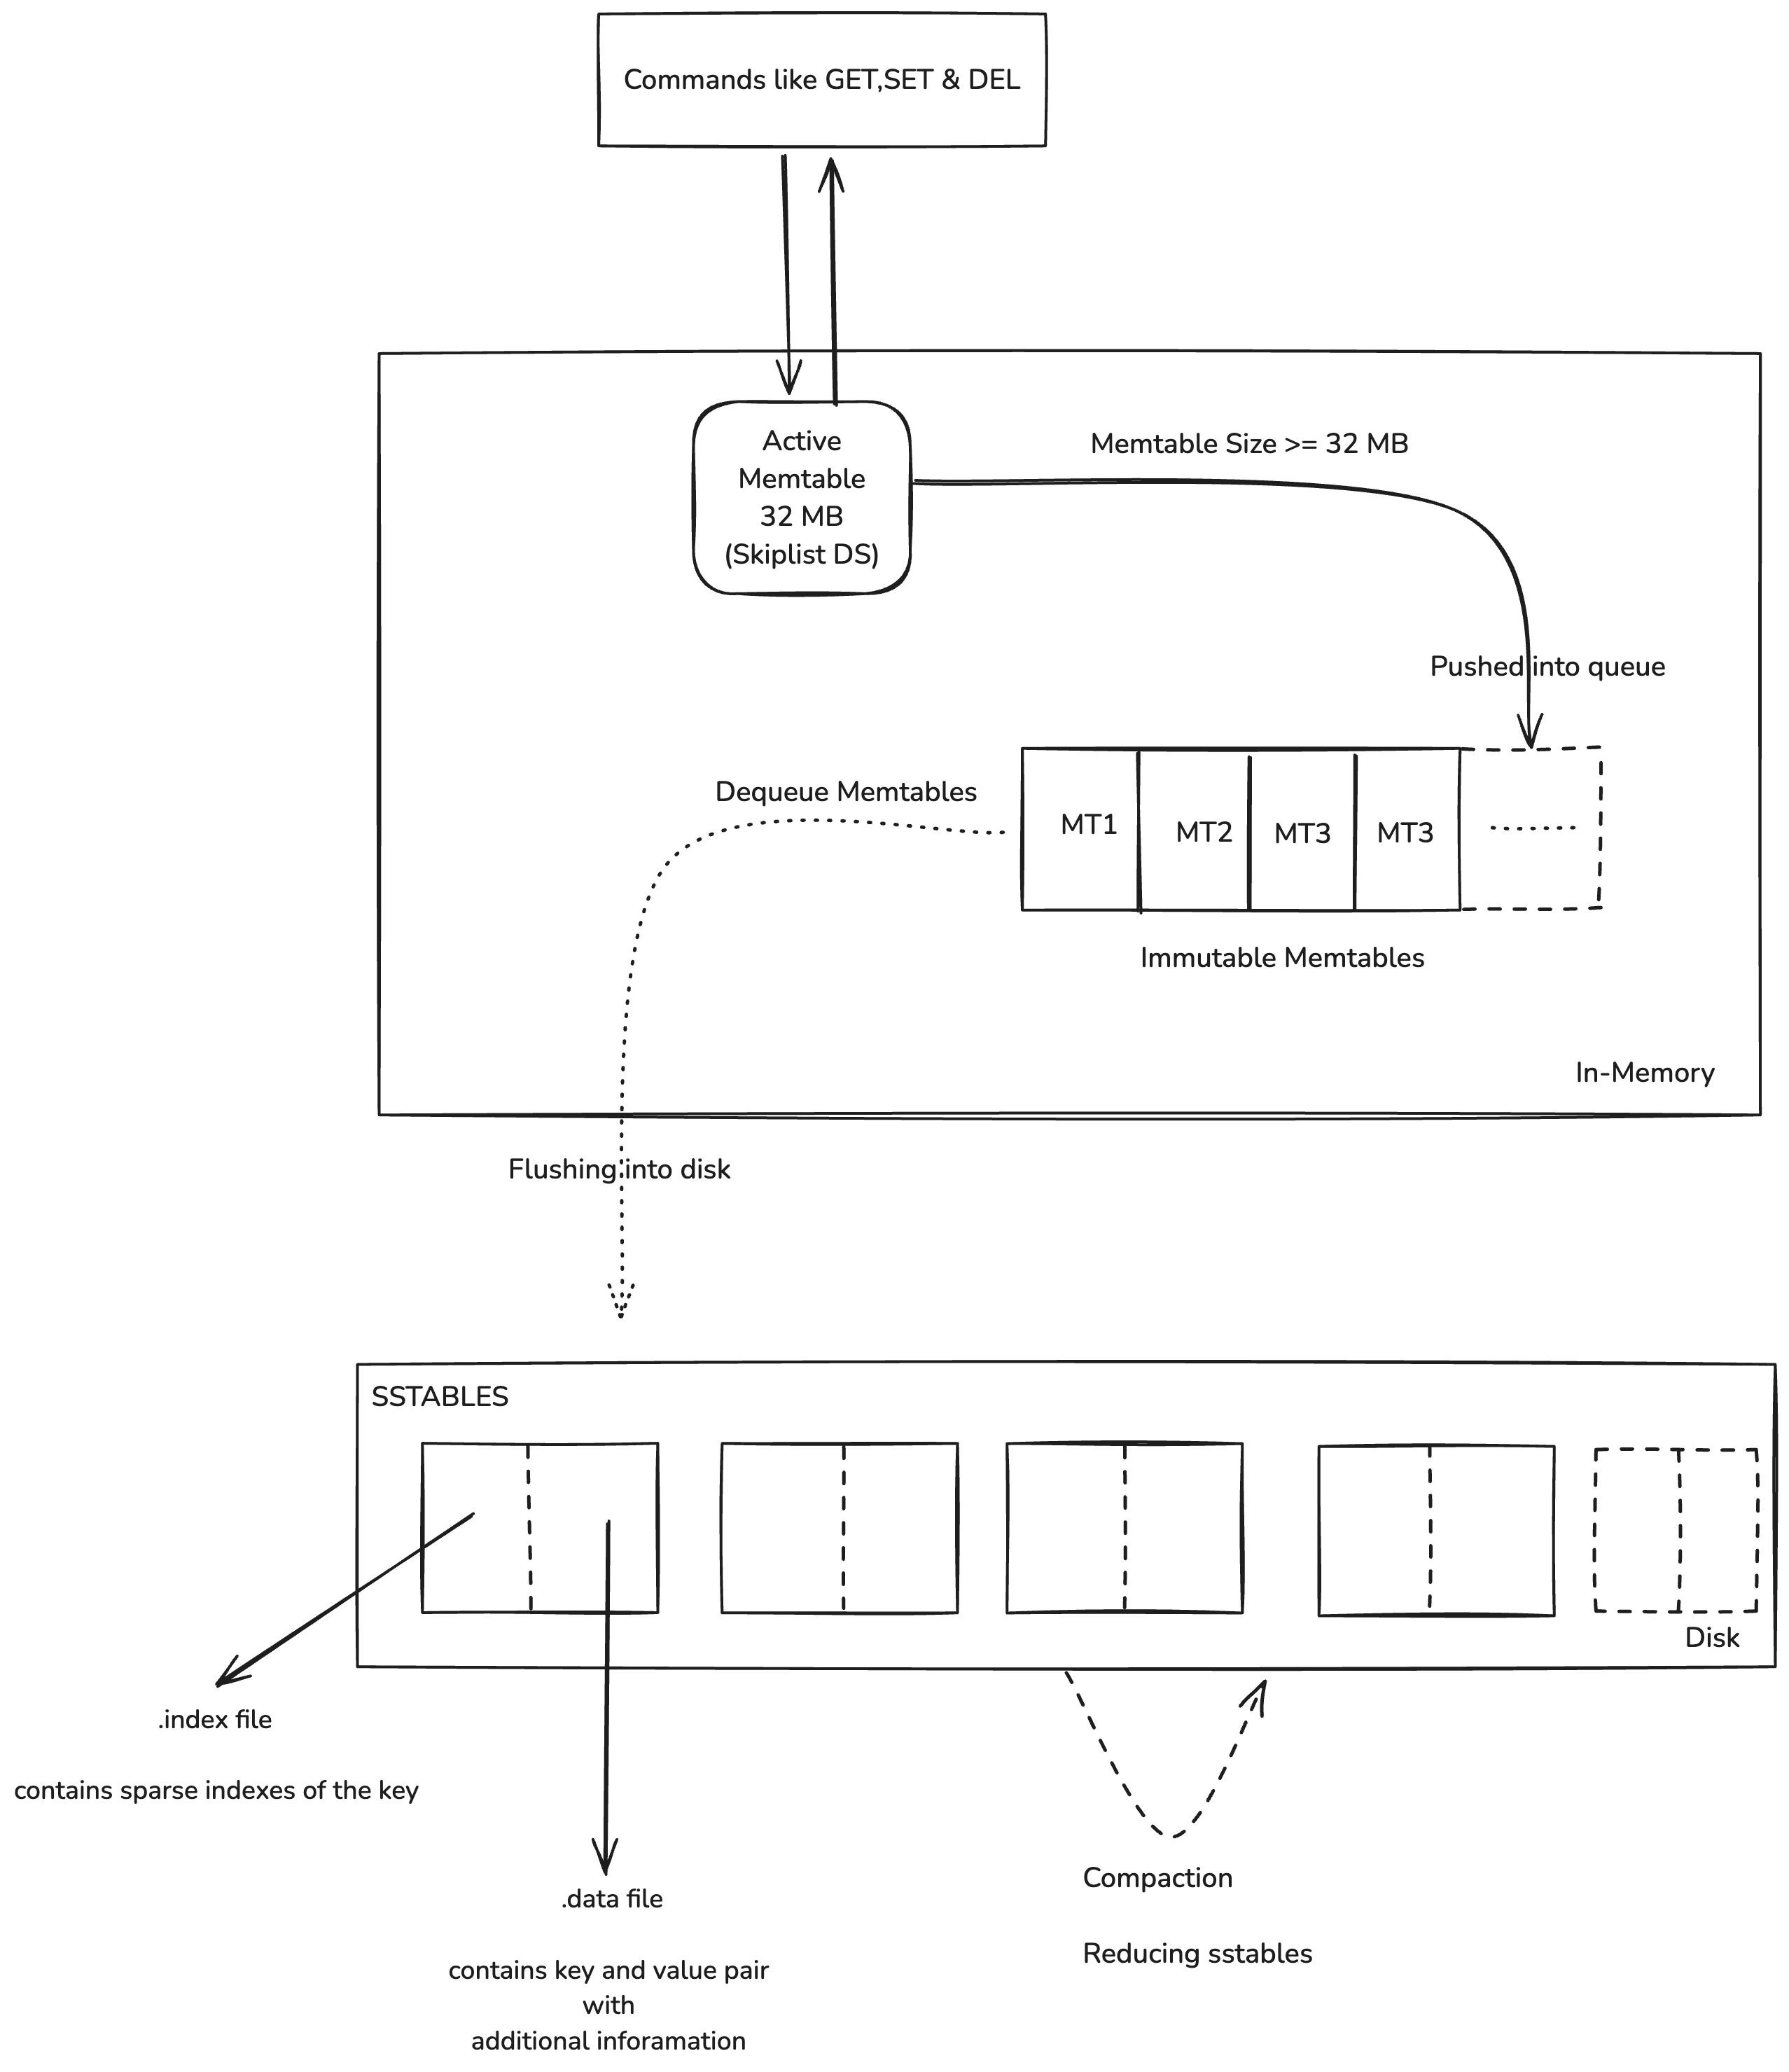
\includegraphics[width=0.8\textwidth]{./pictures/LSM Tree.png}
\caption{Overall working of the LSM Tree}
\label{fig:lsm_tree}
\end{figure}

To understand the overall working of the LSM tree, let's discuss about each operation in detail so that we can understand how the LSM tree works.

\subsubsection{Insertion}

\noindent The insertion operation works as follows in the LSM tree:
\begin{itemize}
    \item First, the key-value pair is inserted into the MemTable. The MemTable is a skip list that stores the data in sorted order.
    \item If the MemTable reaches a certain size (in this case, 32MB), it is marked as immutable and added into the list of immutable MemTables and a new MemTable is created.
    \item Now in the background there is a thread which periodically flushes the immutable MemTables to disk as SSTables. This is done to ensure that the data is stored in the disk.
    \item Now as the memtable is a skiplist which is already sorted, the data is written to the SSTable in sorted order. Two files are created for each SSTable: the data file and the index file.
    \item The data file contains the actual key-value pairs stored in sorted order, while the index file contains the sparse indexes of key-value pairs.
    \item The index file is used to quickly locate the data file, as it contains the offsets of the key-value pairs in the data file.
\end{itemize}

\noindent Before understanding search operation, let's discuss about the deletion operation.

\subsubsection{Deletion}
\noindent The deletion is somewhat a special case of insertion. In this case, we will insert a special key-value pair with the value as \textbf{TOMBSTONE} and the key as the key to be deleted.

\noindent Why not a normal deletion? There are two reasons for this:
\begin{itemize}
    \item The LSM tree is designed to be immutable, meaning that once data is written to disk, it cannot be modified. This allows for efficient reads and writes, as the data is stored in a sorted order.
    \item Lets say you have a key with k1 which is in SSTable 1 after sometime you modify the value of k1 which is in memtable not yet flushed to disk. Now if you delete the key k1, the value of k1 in SSTable 1 will be different from the value of k1 in the memtable. This will cause inconsistency in the data.
\end{itemize}

\noindent You may ask what is the use inserting a special key-value pair with the value as \textbf{TOMBSTONE}. That's where the merge operation comes into play which will be discussed in the next section.

\noindent In my implementation \textbf{TOMBSTONE} value is represented as \texttt{"\texttt{\textbackslash}xFF\texttt{\textbackslash}xFF\texttt{\textbackslash}xFF\texttt{\textbackslash}xFF"} which is a special value that indicates that the key has been deleted. This allows for efficient deletion of keys, as the key can be marked as deleted without actually removing it from the data structure.

\subsubsection{Searching}
\noindent The search operation works as follows in the LSM tree:

\begin{itemize}
    \item First, the key is searched in the MemTable. If the key is found, the value is returned if the value is not \textbf{TOMBSTONE}. If the value is \textbf{TOMBSTONE}, it means that the key has been deleted and a null value is returned.
    \item If the key is not found in the MemTable, the immutable MemTables are searched in reverse order. This is done to ensure that the most recent data is returned. Again if the value is \textbf{TOMBSTONE}, it means that the key has been deleted and a null value is returned.
    \item If the key is not found in the immutable MemTables, the SSTables are searched in reverse order or latest first. This is done to ensure that the most recent data is returned.
    \item The index file is used to quickly locate the data file, as it contains the offsets of the key-value pairs in the data file.
    \item If the key is found in any of the SSTables, the value is returned if the value is not \textbf{TOMBSTONE}. If the value is \textbf{TOMBSTONE}, it means that the key has been deleted and a null value is returned. Since we are searching latest first if the TOMBSTONE is found in the latest SSTable, we can stop searching and return null.
\end{itemize}

\noindent By now you might figured out that lsm-trees are not efficient for read-heavy workloads. This is because the search operation requires searching through multiple data structures (MemTable, immutable MemTables, and SSTables) to find the key-value pair. This means that lsm trees are good for write-heavy workloads but not for read-heavy workloads. This is where the merge operation comes into play. There are so many other optimizations like Bloom filters which are not implemented due to time constraints.

\subsection{Features of LSM Trees}

\subsubsection{Compaction Operation}

\noindent As the SSTables are immutable, they cannot be modified once they are written to disk. This means that if a key is updated, a new SSTable must be created with the updated value. This can lead to multiple SSTables containing the same key with different values. To solve this problem, LSM trees use a compaction operation.

\noindent The compaction operation works as follows:
\begin{itemize}
    \item The compaction operation is performed in the background and is triggered when the number of SSTables exceeds a certain threshold (in this case, 100).
    \item The compaction operation merges multiple SSTables into a single SSTable. This is done to reduce the number of SSTables and to ensure that the data is stored in sorted order.
    \item Also during the compaction if we find any key with the value as \textbf{TOMBSTONE} we will remove that key from the SSTable. This is done to ensure that the data is stored in sorted order and to reduce the size of the SSTable.
    \item During the compaction operation, the key-value pairs are merged and duplicates are removed. If a key is found in multiple SSTables, the most recent value is kept and the others are discarded.
    \item The resulting SSTable is written to disk and replaces the old SSTables.
    \item The old SSTables are deleted to free up space on disk.
    \item The compaction operation is performed in the background to ensure that the system remains responsive and does not block other operations.
    \item The compaction operation is performed in a way that ensures that the data is always stored in sorted order. This allows for efficient reads and writes, as the data is stored in a sorted order.
\end{itemize}

\section{Part B: Server Implementation}

\subsection{System Architecture}

The Blink-DB server is built using an event-driven architecture based on kqueue, which is an efficient I/O event notification mechanism available on BSD-based systems (including macOS). This choice allows the server to handle multiple connections concurrently with a single thread, reducing resource utilization while maintaining high performance.

\noindent The overall architecture consists of the following components:

\begin{itemize}
    \item \textbf{KqueueServer}: Core component that manages the event loop and client connections
    \item \textbf{RESP Protocol Handler}: Handles parsing and encoding of Redis-compatible commands
    \item \textbf{LSM Tree Engine}: The storage engine from Part-A that manages the data
\end{itemize}

\subsubsection{KqueueServer}

The KqueueServer class is the central component of the system, responsible for managing the server socket, setting up the kqueue event notification mechanism, accepting new client connections, reading data from clients, processing client requests, sending responses back to clients, and managing client disconnections.

\noindent The server operates in a non-blocking mode, which means that I/O operations don't block the execution thread. Instead, the kqueue mechanism notifies the server when data is available for reading or when a socket is ready for writing.

\noindent \textbf{Key Components}:

\begin{itemize}
    \item \textbf{Server Socket}: The main socket that listens for incoming connections
    \item \textbf{Kqueue}: The event notification mechanism
    \item \textbf{Event List}: A collection of events that the kqueue is monitoring
    \item \textbf{Client Buffers}: A map that stores the data buffers for each connected client
\end{itemize}

\noindent \textbf{Server Initialization}:

During initialization, the server:
\begin{itemize}
    \item Creates a non-blocking TCP socket
    \item Binds it to the specified address and port
    \item Creates a kqueue instance
    \item Adds the server socket to the kqueue for monitoring read events
    \item Initializes the event list
\end{itemize}

\noindent This setup creates the foundation for handling multiple client connections efficiently without using multiple threads or processes.

\subsection{Event Loop}

The core of the server is the event loop, which continuously waits for events and processes them. The event loop uses the kqueue mechanism to wait for events such as new client connections, client data available for reading, or client disconnections.

\noindent The event loop:
\begin{itemize}
    \item Waits for events using the kqueue system call
    \item Resizes the event list if necessary to accommodate more events
    \item Processes each event based on its type:
    \begin{itemize}
        \item For the server socket: accepts new connections
        \item For client sockets: processes client messages
        \item For error or EOF events: closes the connection
    \end{itemize}
\end{itemize}

\noindent This event-driven approach allows the server to handle thousands of concurrent connections with minimal resource usage, as it doesn't require a separate thread for each connection.

\subsection{Connection Handling}

When a new connection is detected on the server socket, the server accepts the connection, sets it to non-blocking mode, and adds it to the kqueue for monitoring. This process enables the server to receive notifications when data is available for reading from the client.

\noindent The connection handling process includes:
\begin{itemize}
    \item Accepting the new connection with the accept() system call
    \item Setting the client socket to non-blocking mode
    \item Adding the client socket to the kqueue for monitoring read events
    \item Initializing a buffer for storing data received from the client
\end{itemize}

\noindent The accept() call is wrapped in a loop to handle the case where multiple connections arrive simultaneously. The loop continues until accept() returns an error indicating no more connections are pending.

\subsection{Message Processing}

The server uses an efficient approach for reading and processing client messages. When data is available for reading from a client socket, the server reads the data in chunks, appends it to the client's buffer, and tries to parse it as a RESP command.

\noindent The message processing follows these steps:
\begin{itemize}
    \item Reading data from the client socket in chunks
    \item Appending the data to the client's buffer
    \item Ensuring the buffer has sufficient capacity for additional data
    \item When a complete command is received, decoding it using the RESP decoder
    \item Processing the command using the LSM Tree engine
    \item Sending the response back to the client
    \item Clearing the buffer for the next command
\end{itemize}

\noindent The recv() call is wrapped in a loop to read all available data from the client. The loop continues until recv() returns an error indicating no more data is available or until an error occurs.

\subsection{Command Processing}

Once a complete RESP command is received and decoded, the server processes it using the LSM Tree engine from Part-A. The server supports three basic operations:

\begin{itemize}
    \item \textbf{GET}: Retrieve a value for a given key
    \item \textbf{SET}: Store a key-value pair
    \item \textbf{DEL}: Delete a key-value pair
\end{itemize}

\noindent These operations are mapped directly to the corresponding functions in the LSM Tree engine. The results of these operations are then encoded using the RESP protocol and sent back to the client.

\noindent The command processing is wrapped in a try-catch block to handle any exceptions that might occur during the operation. If an exception occurs, an error message is sent to the client, preventing the server from crashing due to client errors.

\section{System Optimizations}

Several optimizations are implemented to maximize the performance of the Blink-DB server:

\begin{itemize}
    \item \textbf{Non-blocking I/O}: All I/O operations are non-blocking, allowing the server to handle multiple clients with a single thread
    \item \textbf{Buffer Management}: Buffers are pre-allocated with \textbf{1MB} size to reduce memory allocation overhead. The server uses a map to manage client buffers, allowing for efficient access and modification
    \item \textbf{Chunked Reading}: Data is read from client sockets in chunks, improving throughput and reducing system call overhead
    \item \textbf{Dynamic Event List Sizing}: The event list size is dynamically adjusted based on the number of concurrent events, optimizing memory usage while ensuring sufficient capacity
\end{itemize}

\noindent These optimizations work together to ensure that the server can handle high throughput and a large number of concurrent connections efficiently.

\section{Integration of Components}

The integration between the LSM-Tree database engine and the kqueue server is seamless:

\begin{itemize}
    \item The server receives commands through the RESP protocol interface
    \item These commands are decoded and mapped to the appropriate LSM-Tree engine operations
    \item Results are encoded back using RESP protocol and sent to clients
    \item The server handles the networking aspects while the LSM-Tree engine manages data storage, retrieval, and organization
\end{itemize}

This separation of concerns allows each component to focus on its specific responsibilities while working together as an integrated system.

\section{Benchmarking}

The benchmark is done with the help of the \textbf{redis-benchmark} tool, which is a built-in benchmarking tool for Redis. It allows you to test the performance of Redis by simulating multiple clients and measuring the throughput and latency of various operations.

\noindent The benchmark is run with the following parameters:
\begin{itemize}
    \item \textbf{Number of requests}: 10000, 100000, 1000000
    \item \textbf{Number of parallel connections}: 10, 100, 1000
    \item \textbf{Data size}: 512 bytes
    \item \textbf{Random key range}: 1024 keys
    \item \textbf{Operations}: SET and GET
\end{itemize}

\begin{table}[htbp]
    \centering
    \caption{Redis Benchmark Results}
    \begin{tabular}{ccccc}
    \toprule
    Concurrent Requests & Parallel Connections & Operation & Throughput (requests/s) & Avg. Latency (ms) \\
    \midrule
    10000 & 10 & SET & 71942.45 & 0.132 \\
    10000 & 10 & GET & 86956.52 & 0.103 \\
    \midrule
    10000 & 100 & SET & 75187.97 & 1.311 \\
    10000 & 100 & GET & 103092.78 & 0.899 \\
    \midrule
    10000 & 1000 & SET & 73529.41 & 12.478 \\
    10000 & 1000 & GET & 90909.09 & 9.853 \\
    \midrule
    100000 & 10 & SET & 74460.16 & 0.128 \\
    100000 & 10 & GET & 91157.70 & 0.095 \\
    \midrule
    100000 & 100 & SET & 76923.08 & 1.293 \\
    100000 & 100 & GET & 94517.96 & 1.000 \\
    \midrule
    100000 & 1000 & SET & 76687.12 & 12.899 \\
    100000 & 1000 & GET & 91659.03 & 10.739 \\
    \midrule
    1000000 & 10 & SET & 73735.44 & 0.129 \\
    1000000 & 10 & GET & 80250.38 & 0.109 \\
    \midrule
    1000000 & 100 & SET & 70766.40 & 1.400 \\
    1000000 & 100 & GET & 86933.84 & 1.084 \\
    \midrule
    1000000 & 1000 & SET & 68465.02 & 14.572 \\
    1000000 & 1000 & GET & 84118.45 & 11.790 \\
    \bottomrule
    \end{tabular}
    \label{tab:redis_benchmark}
\end{table}

\section{Conclusion}

Blink-DB is a comprehensive key-value store database system that combines a write-optimized LSM-Tree storage engine with a high-performance non-blocking server. The integration of these components results in a system that can handle high write throughput while efficiently serving concurrent client requests.

The LSM-Tree storage engine is optimized for write-heavy workloads, allowing for fast inserts and updates. The non-blocking server, built using kqueue, efficiently handles multiple client connections without the overhead of multiple threads or processes.

Together, these components form a robust and scalable database system suitable for applications requiring high write throughput and concurrent access.

\end{document}